\documentclass[12pt,a4paper,oneside]{ctexart}
\usepackage[top=2.0cm, bottom=2.0cm, left=2.8cm, right=2.8cm]{geometry}
\usepackage{graphicx}
\usepackage{array}
\usepackage{tabularx}
\usepackage{longtable}
\usepackage{booktabs}
\usepackage{setspace}
\usepackage{fancyhdr}
\usepackage[compact]{titlesec}
\usepackage{tocloft}
\usepackage{hyperref}
\usepackage{float}
\usepackage{placeins}
\usepackage{enumitem}
\setlist{noitemsep, topsep=2pt, parsep=0pt, partopsep=0pt}
\usepackage{listings}
\usepackage{xcolor}
\usepackage{caption}
\usepackage{amsmath}

\hypersetup{
    colorlinks=true,
    linkcolor=black,
    urlcolor=black,
}

\pagestyle{fancy}
\fancyhf{}
\fancyfoot[C]{\thepage}

\renewcommand{\cfttoctitlefont}{\hfill\Large\bfseries}
\renewcommand{\cftaftertoctitle}{\hfill}

\titleformat{\section}{\Large\bfseries\centering}{\thesection}{1em}{}
\titleformat{\subsection}{\large\bfseries}{\thesubsection}{1em}{}
\titleformat{\subsubsection}{\normalsize\bfseries}{\thesubsubsection}{1em}{}

\setstretch{1.35}

% 紧凑布局设置
\setlength{\parskip}{0.3ex}
\setlength{\floatsep}{6pt plus 2pt minus 2pt}
\setlength{\textfloatsep}{8pt plus 3pt minus 2pt}
\setlength{\intextsep}{6pt plus 2pt minus 2pt}
\setlength{\abovecaptionskip}{4pt}
\setlength{\belowcaptionskip}{4pt}
\setlength{\abovedisplayskip}{4pt plus 2pt minus 2pt}
\setlength{\belowdisplayskip}{4pt plus 2pt minus 2pt}

% 目录紧凑
\setcounter{tocdepth}{2}
\renewcommand{\cftbeforesecskip}{2pt}
\renewcommand{\cftbeforesubsecskip}{2pt}

% 标题紧凑
\titlespacing{\section}{0pt}{8pt plus 2pt minus 2pt}{4pt plus 2pt}
\titlespacing{\subsection}{0pt}{6pt plus 2pt minus 2pt}{3pt plus 2pt}
\titlespacing{\subsubsection}{0pt}{4pt plus 2pt minus 2pt}{2pt plus 2pt}

\newcommand{\covername}[1]{{\fontsize{36pt}{40pt}\selectfont\heiti #1}}
\newcommand{\coversub}[1]{{\fontsize{18pt}{22pt}\selectfont\heiti #1}}

% 代码块样式
\lstset{
    basicstyle=\small\ttfamily,
    columns=flexible,
    breaklines=true,
    frame=single,
    backgroundcolor=\color{gray!5},
    extendedchars=true,
    xleftmargin=1em,
    xrightmargin=1em,
    aboveskip=6pt,
    belowskip=6pt,
}

\begin{document}

% ========== 封面 ==========
\begin{titlepage}
\centering
\vspace*{1.5cm}

\includegraphics[width=4cm]{media/logo.jpeg}
\vspace{0.6cm}

\covername{综合实训报告}
\\[0.3cm]
\coversub{转转校园二手物品交易平台设计与实现}
\\[1.2cm]

\begin{tabular}{>{\kaishu\bfseries\large}l>{\large}l}
  \hline
  姓\hspace{2em}名： & 张可凡 \\[0.5cm]
  学\hspace{2em}号： & 2024307020XXX \\[0.5cm]
  班\hspace{2em}级： & 计科210X班 \\[0.5cm]
  指导老师： & 徐士伟 \\[0.5cm]
  \hline
\end{tabular}

\vfill
{\kaishu\large 中国 武汉}
\\[0.3cm]
{\kaishu\normalsize 二〇二六年七月}
\\[0.2cm]
{\kaishu\normalsize 2026.07}


\end{titlepage}

% ========== 目录 ==========
\tableofcontents
\newpage

% ========== 正文 ==========

% ====== 第1章 实训目的及内容 ======
\section{实训目的及内容}

\subsection{实训目的}

本次综合实训以软件工程理论为指导，通过开发一个完整的校园二手物品交易平台，达到以下目的：

\begin{enumerate}[nosep]
    \item 巩固和深化软件工程、Web前端开发技术、Java程序设计、数据库原理与应用、计算机网络等课程的理论知识。
    \item 掌握前后端分离架构的开发模式，熟悉SpringBoot + Vue3主流技术栈的工程化实践。
    \item 培养团队协作能力与项目管理能力，体验从需求分析、系统设计、编码实现到测试部署的完整软件生命周期。
    \item 提升独立解决实际问题的能力，包括技术选型、架构设计、性能优化、安全防护等综合工程素养。
\end{enumerate}

\subsection{实训内容}

本项目"转转"是一个面向高校学生的C2C二手物品交易Web应用系统，旨在解决校园闲置物品循环利用的需求。系统采用前后端分离架构，后端基于Spring Boot 3.2.0 + Spring Security + JWT + MyBatis-Plus 3.5.5实现RESTful API，JDK 17运行环境；前端基于Vue 3.4 + TypeScript 5.3 + Vite 5 + Element Plus 2.5构建用户界面；使用MySQL 8.0存储业务数据，Redis 7提供缓存加速，全容器化Docker Compose一键部署。

系统实现了完整的交易闭环，包括用户管理、商品管理、购物车与订单交易、站内消息沟通、后台管理五大核心模块，共计60余个RESTful API和20余个前端页面，并提供Docker Compose一键部署方案。

\subsection{实训安排}

\subsubsection{团队组成}

实训小组共5人，分工如表1所示：

\begin{table}[htbp]
\centering
\caption{团队成员与角色分工}
\label{tab:team}
\small
\begin{tabular}{|c|c|p{4.5cm}|}
\hline
\textbf{成员} & \textbf{角色} & \textbf{职责} \\
\hline
张可凡（队长） & 全栈/项目管理 & Docker部署、管理后台前端、Postman测试、文档整合 \\
\hline
阮崇轩 & 前端开发 & 前端工程搭建、用户认证模块、消息通知系统、UI动效与交互优化 \\
\hline
刘轩霆 & 后端开发A & 用户模块、商品模块、安全框架、订单核心流程、后台管理API \\
\hline
胡欣悦 & 后端开发B & 购物车模块、消息与通知模块、数据统计、文件上传、Docker部署运维 \\
\hline
李硕 & 前端开发 & 首页与商品模块、购物车与订单页面、管理后台页面、数据可视化 \\
\hline
\end{tabular}
\end{table}

\subsubsection{开发计划}

项目周期为2026年7月4日至2026年7月10日，共分四个阶段：

\begin{itemize}[nosep]
    \item \textbf{第1天（7月4日）}：环境搭建与基础框架——Git仓库创建、Docker编排、前后端项目脚手架、数据库表设计。
    \item \textbf{第2--3天（7月5日--6日）}：核心功能开发（用户+商品）——安全框架集成、注册登录、商品CRUD、分类与收藏。
    \item \textbf{第4--5天（7月7日--8日）}：核心功能开发（订单+消息）——购物车、订单状态流转、站内信、系统通知。
    \item \textbf{第6--7天（7月9日--10日）}：管理后台 + 联调测试——用户/商品/订单管理、数据统计、全量接口联调、文档编写。
\end{itemize}

% ====== 第2章 需求分析 ======
\section{需求分析}

转转校园二手交易平台作为面向高校学生的C2C交易平台，主要服务三类用户角色：游客（未登录用户）、普通用户（买家和卖家双重身份）以及管理员。系统的顶层用例如图\ref{fig:usecase}所示。

\begin{figure}[ht!]
\centering
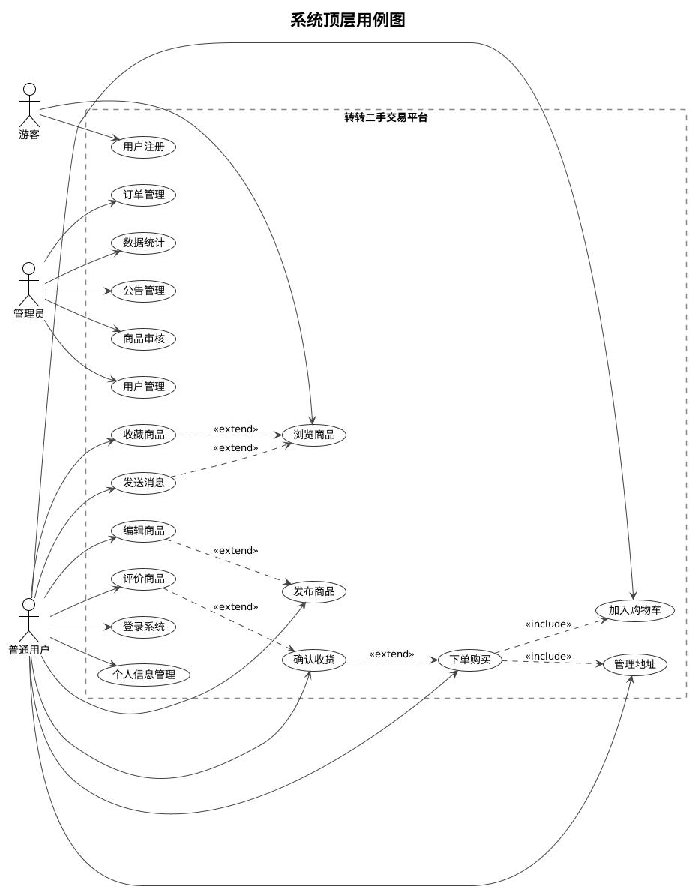
\includegraphics[width=0.85\textwidth]{media/usecase_plantuml.pdf}
\caption{系统顶层用例图}
\label{fig:usecase}
\end{figure}

\FloatBarrier
\subsection{功能需求}

系统包含以下五大核心功能模块：

\subsubsection{用户管理模块}

支持用户的完整生命周期管理。游客可通过邮箱/手机号验证码注册成为平台用户，注册后可使用用户名或邮箱或手机号登录系统。系统采用JWT双Token机制（Access Token 2小时过期，Refresh Token 7天过期）实现无状态认证，支持密码找回、Token无感刷新、安全退出（Token加入Redis黑名单）等功能。用户可在个人中心编辑昵称、简介、性别，上传头像，管理多个收货地址并设置默认地址。

\subsubsection{商品管理模块}

支持商品的完整生命周期管理。卖家可发布商品，填写标题、描述（富文本）、价格、原价、成色，选择分类并上传多张图片。商品发布后需管理员审核方可上架展示。买家可通过首页推荐、分类导航、关键词搜索（全文索引）浏览商品，支持按分类、价格区间、成色筛选，按价格、时间、热度排序。买家可收藏感兴趣的商品，卖家可查看和管理自己发布的商品。

\subsubsection{订单交易模块}

实现完整的交易闭环。买家可将商品加入购物车统一结算，下单时选择收货地址。订单状态按"待付款$\to$待发货$\to$待收货$\to$已完成"流转，系统提供模拟支付功能，卖家可录入物流信息发货，买家确认收货后可对交易进行评分和评价。所有状态变更均记录订单日志，便于追踪溯源。

\subsubsection{消息与通知模块}

支持买卖双方的即时沟通。买家可通过商品详情页的"联系卖家"发起会话，双方可互发文本消息或图片消息，支持会话列表查看、聊天记录分页查询、消息已读/未读标记和未读计数。系统自动推送订单状态变更、审核结果等系统通知。

\subsubsection{后台管理模块}

为管理员提供全面的管理功能。包括用户管理（用户列表、搜索筛选、禁用/启用、修改角色）、商品审核（待审核列表、审核通过/驳回、违规强制下架）、订单管理（按状态/单号/日期查询、异常状态处理）、数据统计（注册用户量、商品发布量、成交量、分类占比饼图、趋势折线图，基于ECharts实现）以及公告管理（发布/编辑/删除系统公告）。

\subsection{非功能需求}

\begin{itemize}[nosep]
    \item \textbf{安全性}：密码BCrypt加密存储，JWT双Token无状态认证，接口RBAC权限控制，SQL注入防护（排序字段白名单校验），Nginx安全响应头配置（X-Frame-Options/XSS-Protection/Content-Type-Options），API限流防护（全局30r/s、登录接口10r/m）。
    \item \textbf{性能}：Redis缓存验证码、黑名单Token及热点商品数据，数据库4个复合索引优化高频查询，N+1查询问题修复，前端Gzip压缩与路由懒加载。
    \item \textbf{可用性}：响应式UI设计兼容移动端与桌面端，统一异常处理与友好的错误提示，Token自动刷新机制保证会话连续性，Docker Compose一键部署与恢复。
    \item \textbf{可维护性}：前后端分离架构，RESTful API规范，Knife4j自动生成接口文档，统一返回结果封装，完善的订单日志审计。
\end{itemize}

\FloatBarrier
% ====== 第3章 系统设计 ======
\section{系统设计}

\subsection{体系结构设计}

系统采用前后端分离的B/S架构，前端与后端通过RESTful API进行数据交互。整体架构分为四层，如图\ref{fig:architecture}所示。

\begin{figure}[ht!]
\centering
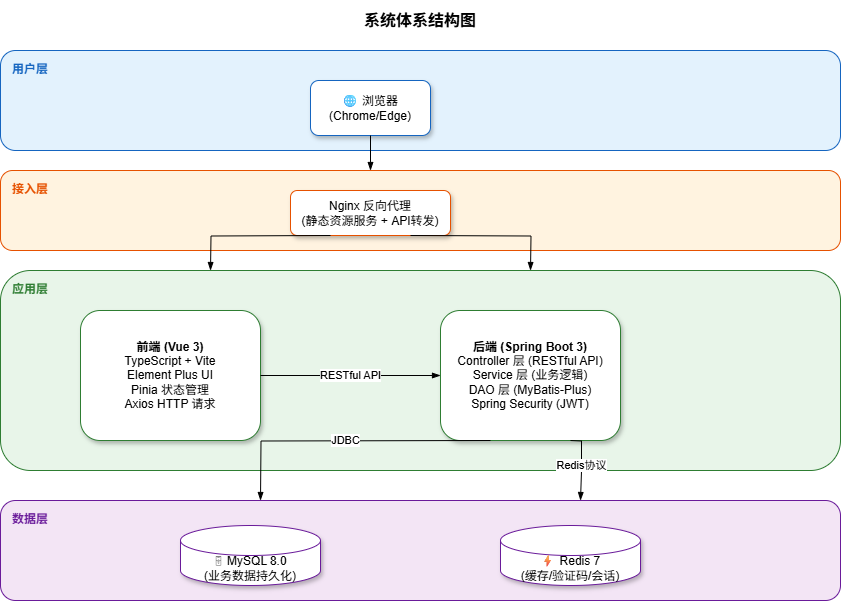
\includegraphics[width=0.82\textwidth]{media/architecture.png}
\caption{系统体系结构图}
\label{fig:architecture}
\end{figure}

\FloatBarrier
\subsubsection{前端架构}

前端基于Vue 3.4 + TypeScript 5.3 + Vite 5构建，采用组合式API（Composition API）开发模式。使用Element Plus 2.5提供UI组件库，Pinia 2.1（结合持久化插件pinia-plugin-persistedstate）管理全局状态，Vue Router 4.2实现路由控制，共配置21条路由，全部采用懒加载方式。Axios封装请求拦截器自动携带JWT Token，响应拦截器统一处理错误并支持Token无感自动刷新。前端构建通过unplugin-auto-import和unplugin-vue-components实现Element Plus按需自动导入，使用vite-plugin-compression开启Gzip压缩。

\subsubsection{后端架构}

后端采用Spring Boot 3.2.0 + MyBatis-Plus 3.5.5 + Spring Security技术栈，JDK 17运行环境，遵循经典的三层架构设计：

\begin{itemize}[nosep]
    \item \textbf{Controller层}：接收HTTP请求，参数校验，调用Service层处理业务，返回统一封装的Result对象。API文档通过Knife4j（Swagger增强）自动生成。
    \item \textbf{Service层}：业务逻辑处理，包括用户认证、商品管理、订单流转、消息通信等核心业务。
    \item \textbf{DAO层}：基于MyBatis-Plus操作数据库，支持LambdaQueryWrapper动态条件查询和MyBatis-Plus分页插件。
\end{itemize}

安全方面，Spring Security配置为无状态会话模式，通过JwtAuthenticationFilter拦截请求，从请求头提取Token，验证有效性并检查Redis黑名单后设置SecurityContext。项目使用Hutool工具库（5.8.25）提供通用工具方法，Lombok简化实体代码。

\subsubsection{部署架构}

系统采用Docker Compose编排五容器架构：Nginx（前端静态资源服务与反向代理，映射端口3000）、Spring Boot后端、MySQL 8.0数据库、Redis 7缓存以及phpMyAdmin数据库管理工具（映射端口3001）。所有服务通过内部桥接网络通信，MySQL和Redis不对外暴露端口，后端仅通过Nginx反向代理对外暴露。使用数据卷持久化MySQL数据和Redis数据，确保容器重启不丢失。

\subsection{功能设计}

系统五大核心功能模块之间相互协作，共同构成完整的交易闭环。模块之间的调用关系如图\ref{fig:module-relation}所示。

\begin{figure}[ht!]
\centering
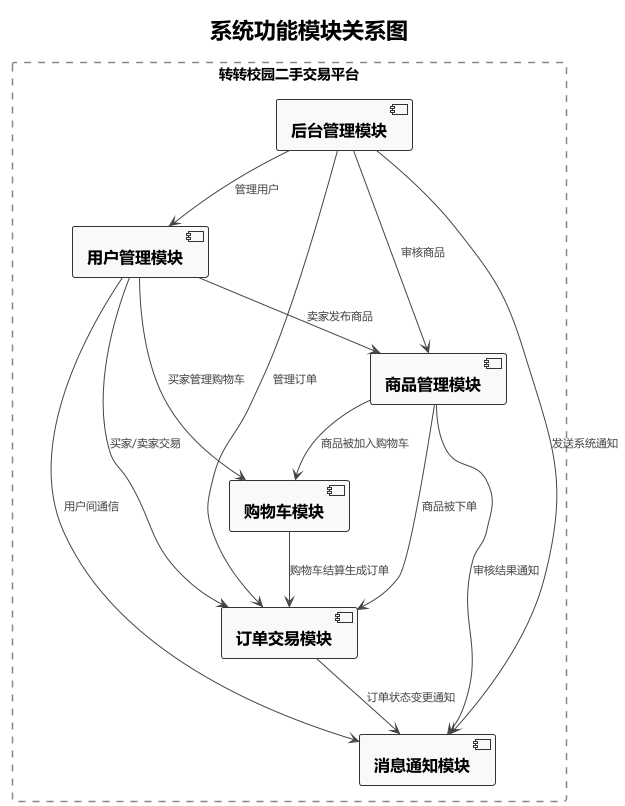
\includegraphics[width=0.75\textwidth]{media/module-relation.png}
\caption{功能模块关系图}
\label{fig:module-relation}
\end{figure}

\FloatBarrier
\subsubsection{用户认证模块流程}

用户认证模块涵盖注册、登录、Token刷新、密码找回、退出登录等核心流程。用户注册后获取JWT双Token，后续请求携带Access Token访问受保护资源，Token过期后由Refresh Token无感刷新。图\ref{fig:swimlane-auth}展示了用户认证的完整流程。

\begin{figure}[ht!]
\centering
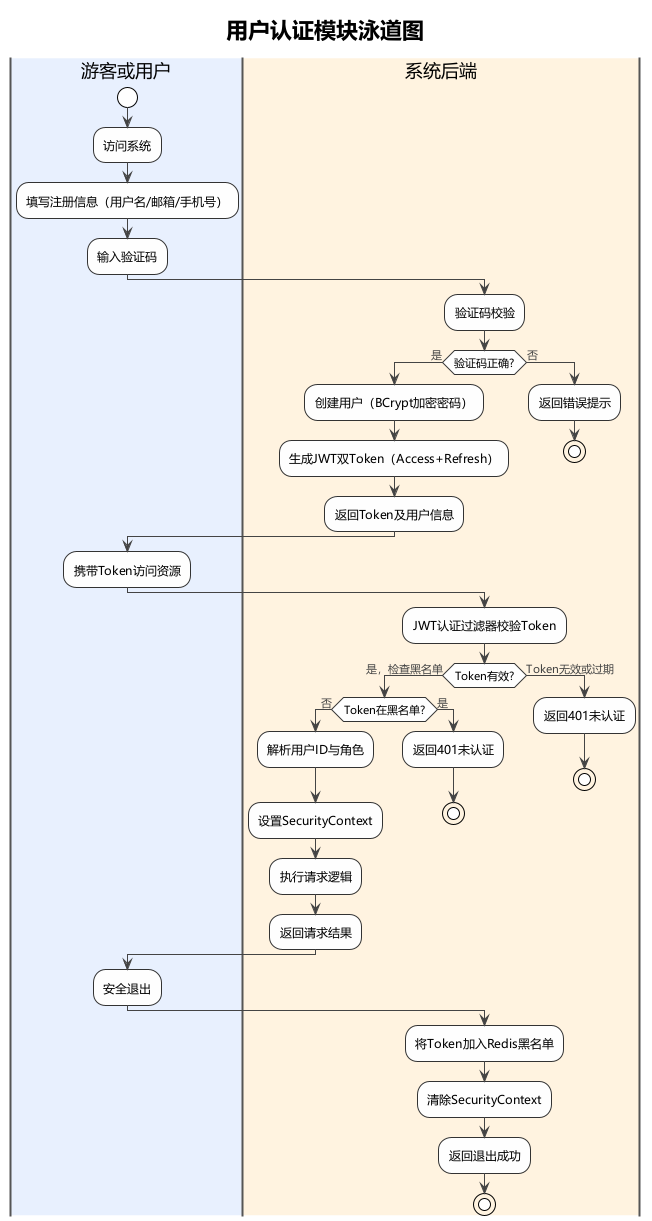
\includegraphics[width=0.85\textwidth,height=0.65\textheight,keepaspectratio]{media/swimlane-auth.png}
\caption{用户认证模块泳道图}
\label{fig:swimlane-auth}
\end{figure}

\FloatBarrier
\subsubsection{商品管理模块流程}

商品管理模块支持商品的完整生命周期——卖家发布商品后需管理员审核方可上架，买家通过搜索、分类浏览、收藏等方式发现商品。图\ref{fig:swimlane-product}展示了商品从发布到上架的跨角色协作流程。

\begin{figure}[ht!]
\centering
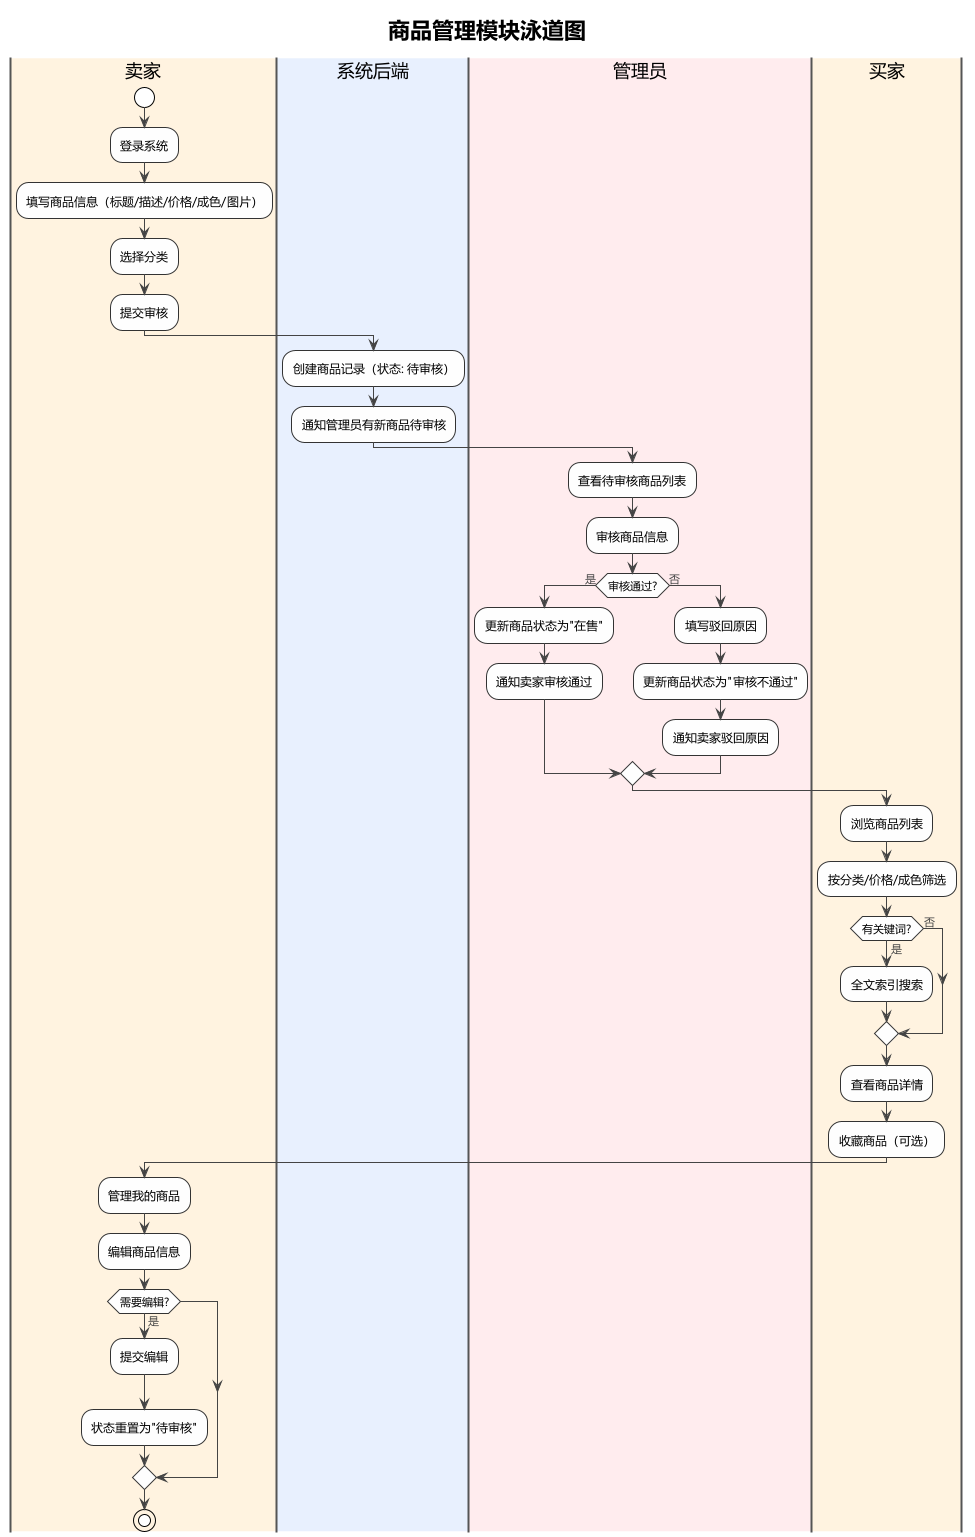
\includegraphics[width=0.85\textwidth,height=0.65\textheight,keepaspectratio]{media/swimlane-product.png}
\caption{商品管理模块泳道图}
\label{fig:swimlane-product}
\end{figure}

\FloatBarrier
\subsubsection{订单交易模块流程}

订单交易模块实现了从购物车、下单、支付、发货、收货到评价的完整交易闭环。买卖双方围绕订单状态流转进行协作，所有状态变更均记录订单日志。图\ref{fig:swimlane-order}展示了订单交易的跨角色流程。

\begin{figure}[ht!]
\centering
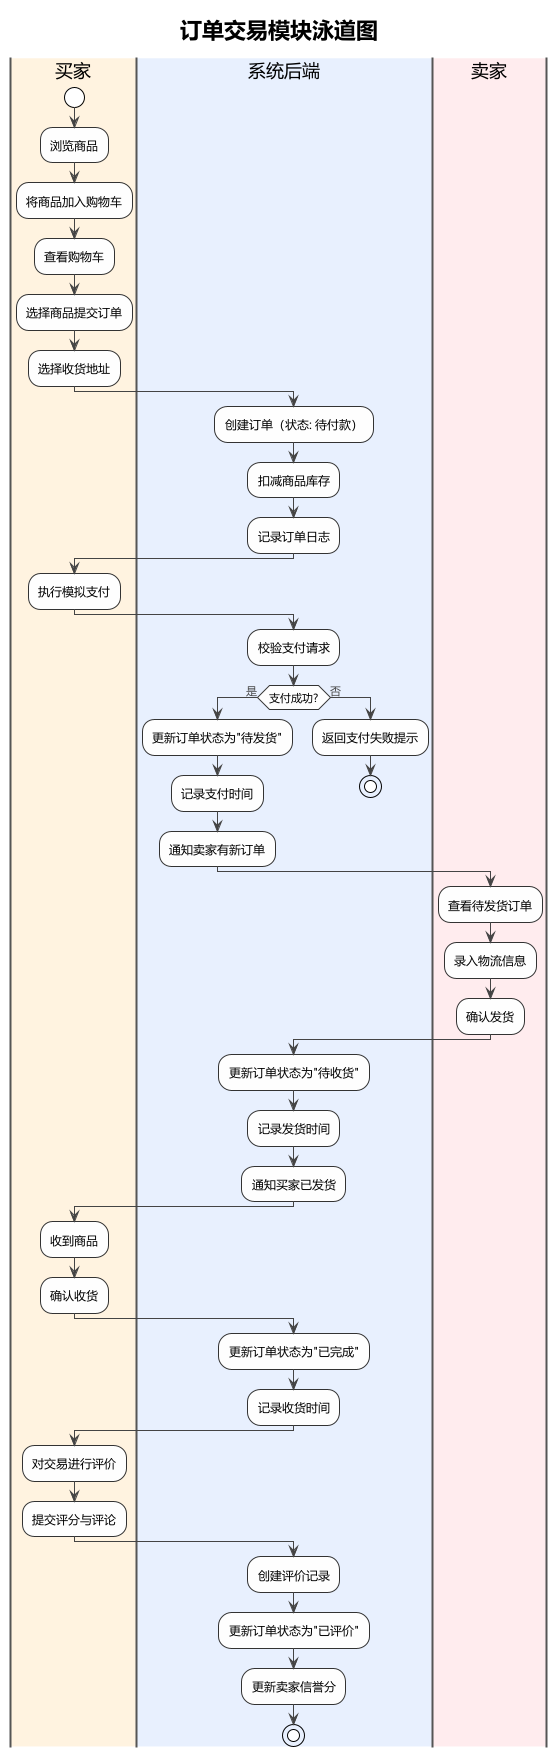
\includegraphics[width=0.85\textwidth,height=0.6\textheight,keepaspectratio]{media/swimlane-order.png}
\caption{订单交易模块泳道图}
\label{fig:swimlane-order}
\end{figure}

\FloatBarrier
\subsubsection{消息通知模块流程}

消息通知模块支持买卖双方之间的站内即时通信，以及系统向用户推送订单状态变更、审核结果等通知。图\ref{fig:swimlane-message}展示了消息发送与通知推送的流程。

\begin{figure}[ht!]
\centering
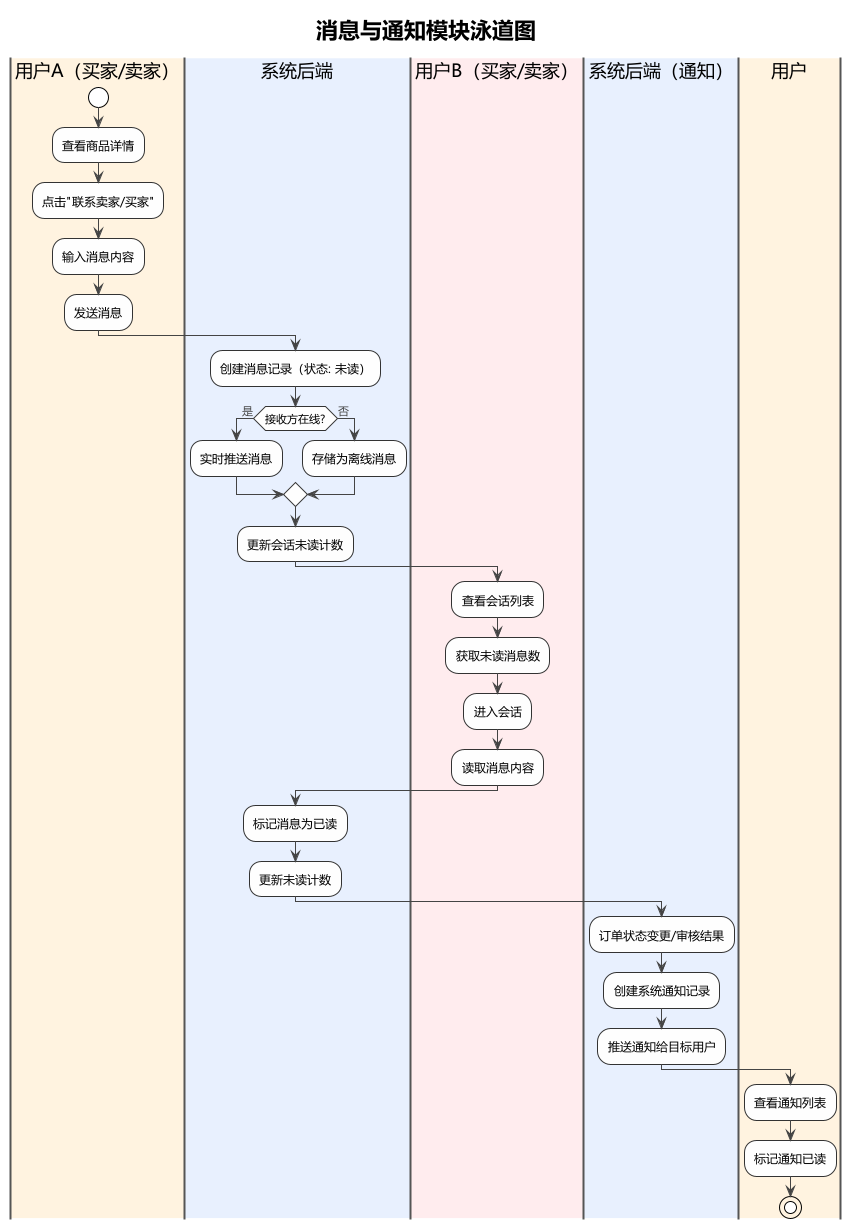
\includegraphics[width=0.85\textwidth,height=0.65\textheight,keepaspectratio]{media/swimlane-message.png}
\caption{消息通知模块泳道图}
\label{fig:swimlane-message}
\end{figure}

\FloatBarrier
\subsubsection{后台管理模块流程}

后台管理模块为管理员提供用户管理、商品审核、订单管理、数据统计和公告管理等全面管理功能。图\ref{fig:swimlane-admin}展示了管理员执行审核与管理的流程。

\begin{figure}[ht!]
\centering
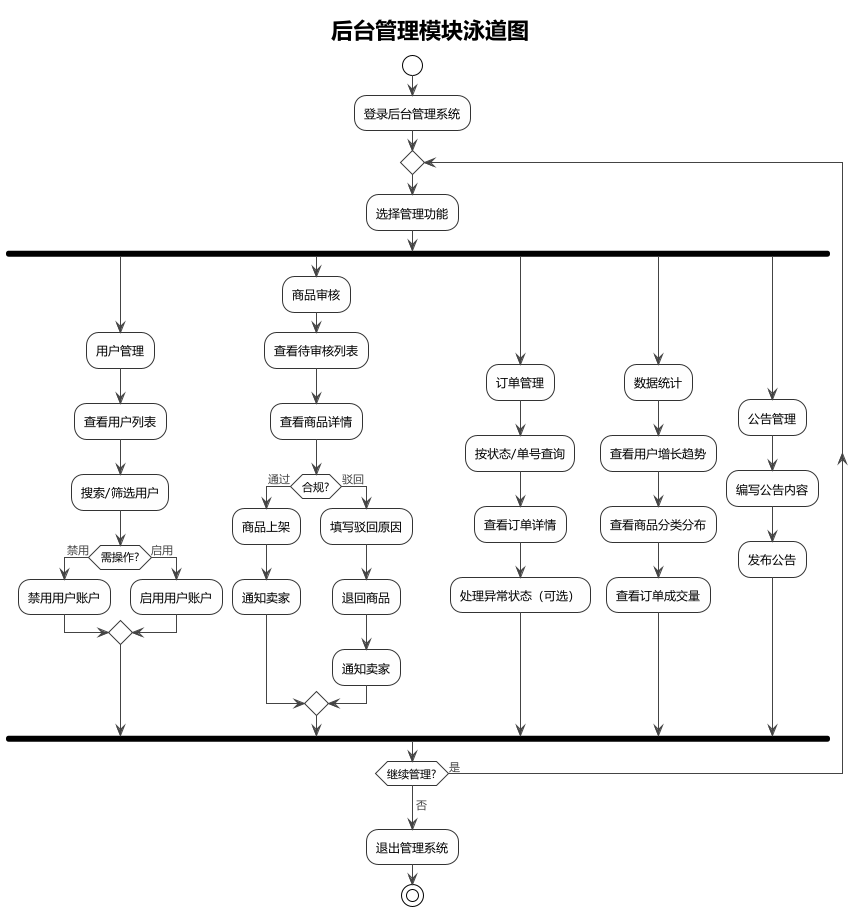
\includegraphics[width=0.85\textwidth,height=0.65\textheight,keepaspectratio]{media/swimlane-admin.png}
\caption{后台管理模块泳道图}
\label{fig:swimlane-admin}
\end{figure}

\FloatBarrier
\subsection{数据设计}

系统共设计13张核心业务表，涵盖用户、商品、订单、消息等全部业务实体。表结构和关系如图\ref{fig:er}所示。

\begin{figure}[ht!]
\centering
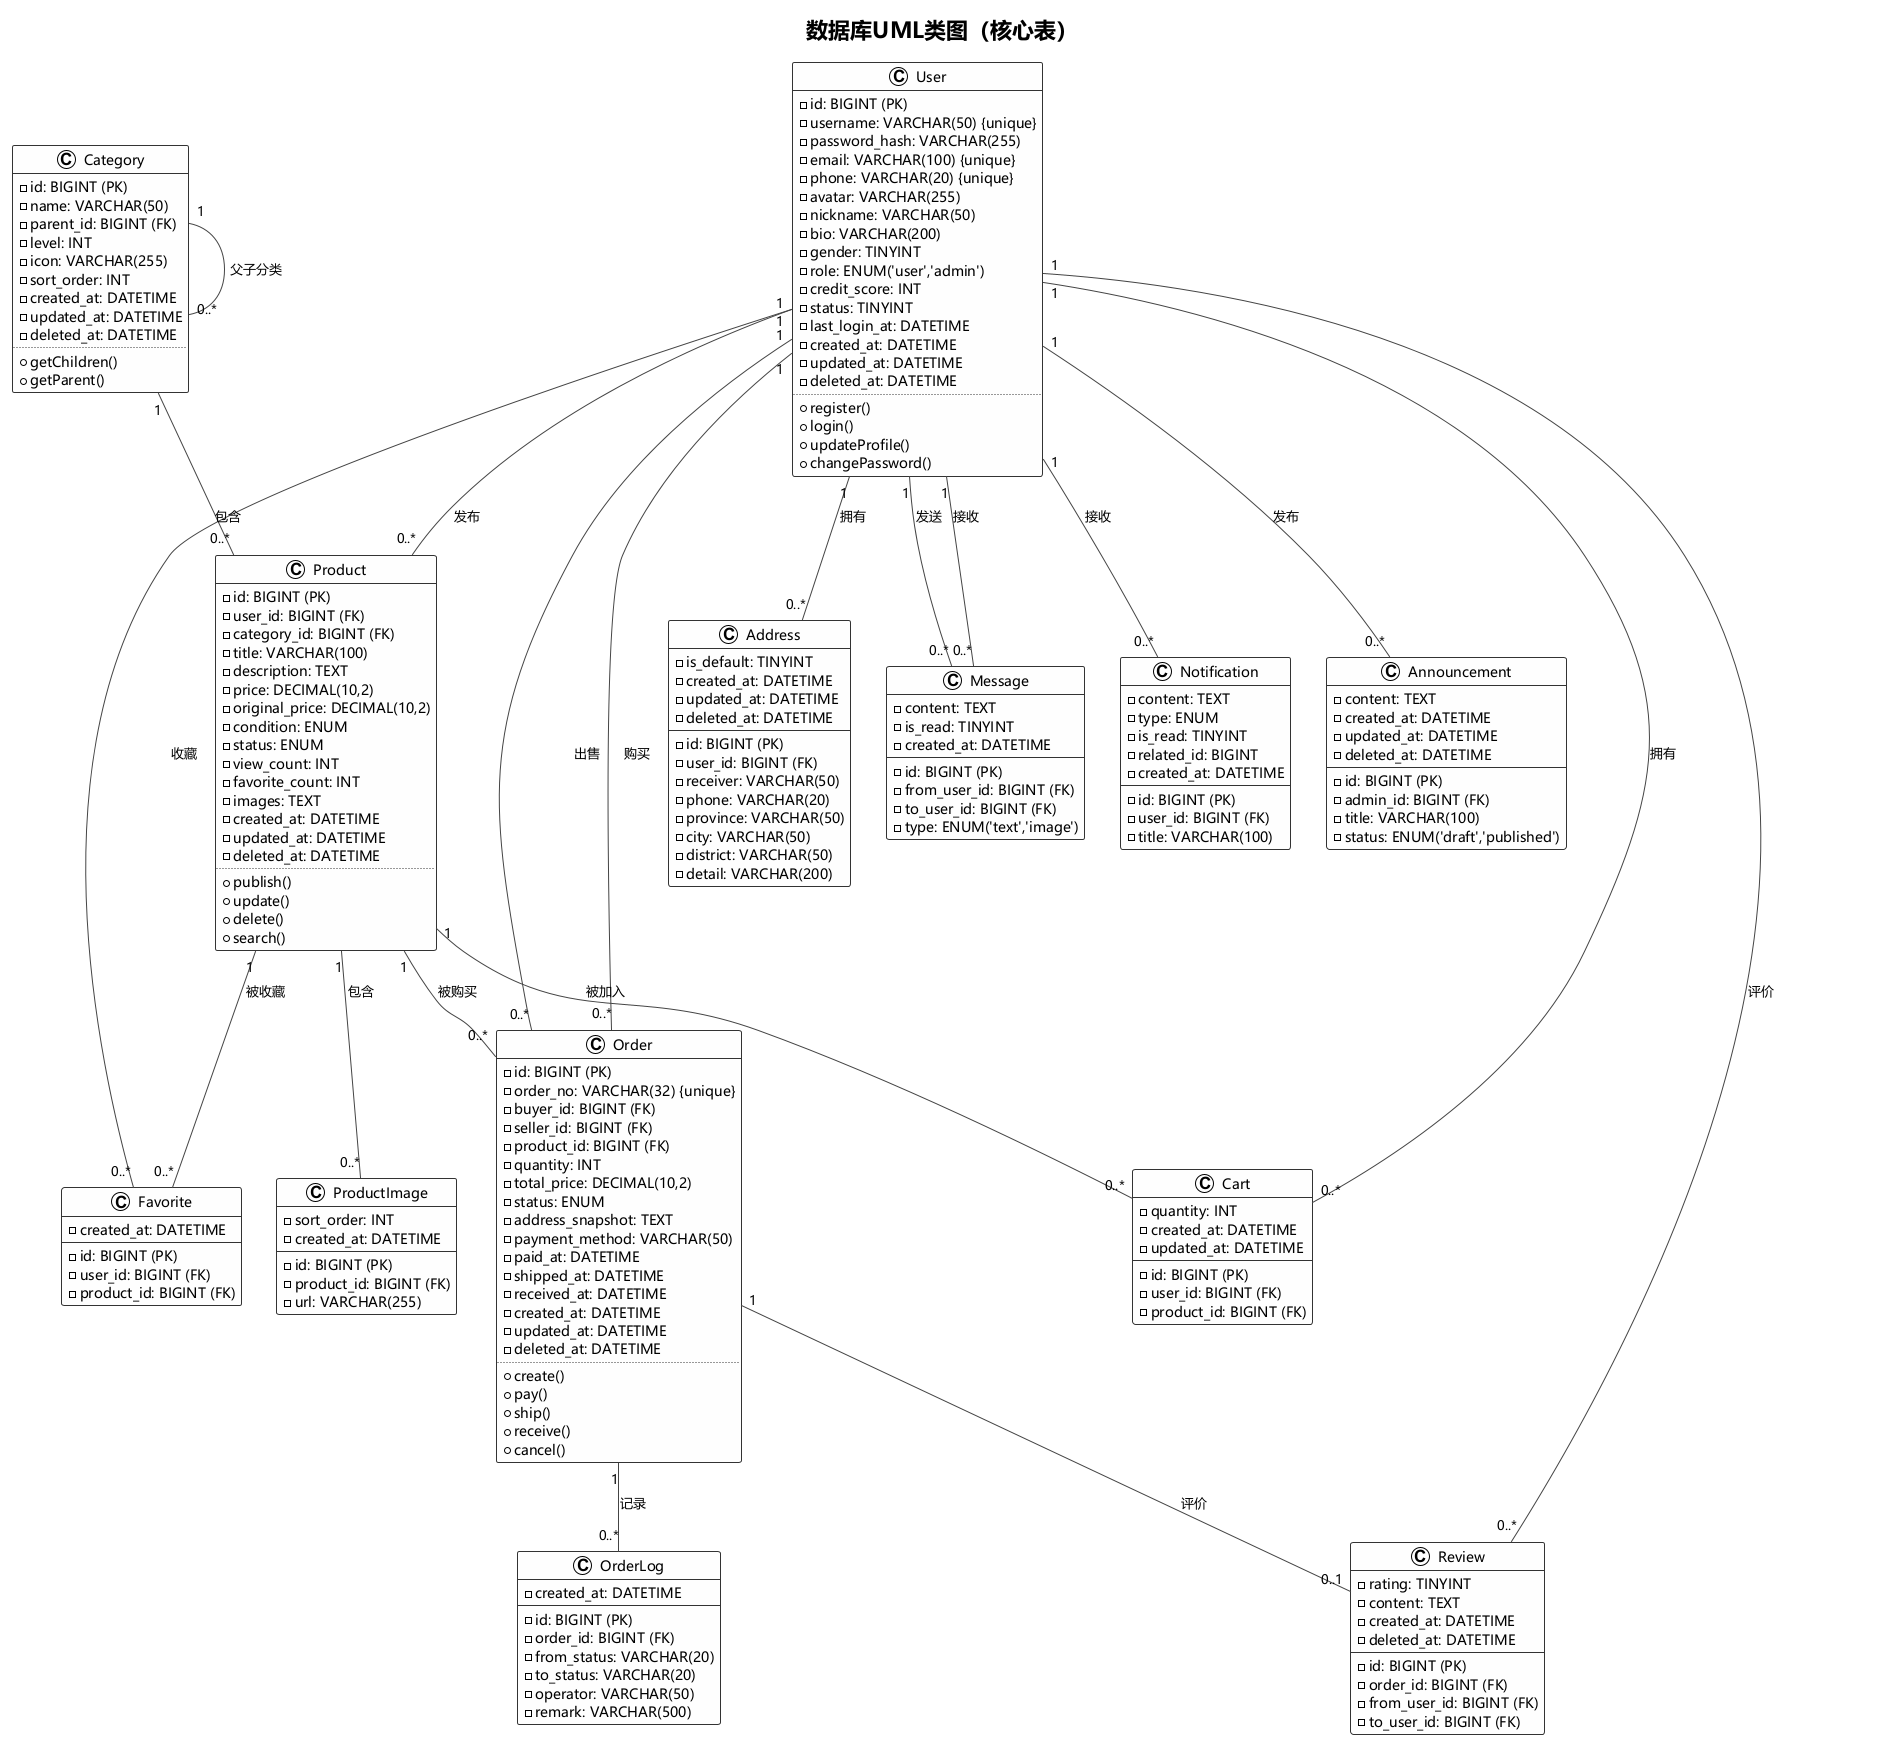
\includegraphics[width=0.85\textwidth,height=0.7\textheight,keepaspectratio]{media/er_uml.png}
\caption{数据库UML类图（核心表）}
\label{fig:er}
\end{figure}

\FloatBarrier
\subsubsection{核心数据库表}

\begin{table}[htbp]
\centering
\caption{核心数据库表清单}
\label{tab:tables}
\small
\begin{tabular}{|p{2.5cm}|p{2.5cm}|p{6.5cm}|}
\hline
\textbf{表名} & \textbf{用途} & \textbf{关键字段} \\
\hline
user & 用户表 & username, password\_hash, email, phone, role \\
\hline
category & 商品分类表 & name, parent\_id, level \\
\hline
product & 商品表 & user\_id, category\_id, title, price, status \\
\hline
product\_image & 商品图片表 & product\_id, url, sort\_order \\
\hline
address & 收货地址表 & user\_id, receiver, phone, province, city \\
\hline
order & 订单表 & order\_no, buyer\_id, seller\_id, status \\
\hline
order\_log & 订单日志表 & order\_id, from\_status, to\_status \\
\hline
cart & 购物车表 & user\_id, product\_id, quantity \\
\hline
message & 消息表 & from\_user\_id, to\_user\_id, content, type \\
\hline
favorite & 收藏表 & user\_id, product\_id \\
\hline
review & 评价表 & order\_id, from\_user\_id, rating \\
\hline
notification & 通知表 & user\_id, title, content, type \\
\hline
announcement & 公告表 & admin\_id, title, content, status \\
\hline
\end{tabular}
\end{table}

数据表设计特点：所有表使用InnoDB引擎和utf8mb4字符集；采用软删除策略（deleted\_at字段配合MyBatis-Plus @TableLogic）；created\_at和updated\_at通过MyMetaObjectHandler自动填充；product表含全文索引支持商品搜索；通过复合索引优化消息会话查询、未读计数、收藏排序等高频查询场景。

\FloatBarrier
% ====== 第4章 系统实现 ======
\section{系统实现}

\subsection{JWT双Token认证机制}

系统采用Access Token + Refresh Token双Token机制实现无状态认证。Access Token有效期为2小时，存储用户ID和角色信息；Refresh Token有效期为7天，用于无感刷新Token。

\begin{lstlisting}[caption=JWT认证过滤器核心逻辑, language=Java]
@Override
protected void doFilterInternal(HttpServletRequest request,
        HttpServletResponse response, FilterChain filterChain)
        throws ServletException, IOException {
    String token = extractToken(request);
    if (StringUtils.hasText(token) && jwtUtil.validateToken(token)
            && !jwtUtil.isRefreshToken(token)) {
        Long userId = jwtUtil.getUserIdFromToken(token);
        // check blacklist
        String tokenId = jwtUtil.getTokenId(token);
        if (tokenId != null && Boolean.TRUE.equals(
                redisTemplate.hasKey("blacklist:token:" + tokenId))) {
            filterChain.doFilter(request, response);
            return;
        }
        // reload user from database for role verification
        User user = userMapper.selectById(userId);
        if (user == null || user.getStatus() == 0) {
            filterChain.doFilter(request, response);
            return;
        }
        // set authentication with DB role
        UsernamePasswordAuthenticationToken authentication =
                new UsernamePasswordAuthenticationToken(
                    userId, null,
                    Collections.singletonList(
                        () -> "ROLE_" + user.getRole().toUpperCase()));
        SecurityContextHolder.getContext()
                .setAuthentication(authentication);
    }
    filterChain.doFilter(request, response);
}

private String extractToken(HttpServletRequest request) {
    String bearerToken = request.getHeader("Authorization");
    if (StringUtils.hasText(bearerToken)
            && bearerToken.startsWith("Bearer ")) {
        return bearerToken.substring(7);
    }
    return null;
}
\end{lstlisting}

\subsection{订单状态流转引擎}

订单模块是整个系统的核心业务，涉及多个状态的流转和数据一致性。采用状态模式设计，每个状态变更均记录订单日志（order\_log表），关键操作（创建订单扣减库存）通过@Transactional保证原子性。此外，系统采用模拟支付流程，无需接入真实第三方支付即可完整体验交易闭环。

\begin{figure}[ht!]
\centering
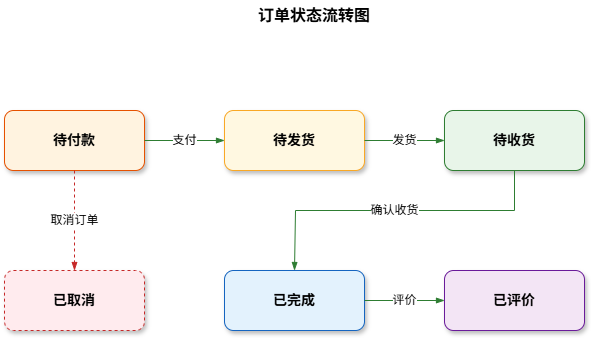
\includegraphics[width=0.62\textwidth]{media/order-flow.png}
\caption{订单状态流转图}
\label{fig:order-flow}
\end{figure}

订单状态流转路径为：

\begin{center}
\textbf{待付款$\xrightarrow{\text{支付}}$待发货$\xrightarrow{\text{发货}}$待收货$\xrightarrow{\text{收货}}$已完成$\xrightarrow{\text{评价}}$已评价}
\end{center}

\subsection{商品搜索与筛选}

商品模块支持多条件组合查询，包括分类筛选、价格区间、成色筛选、关键词搜索以及按价格/时间/热度排序。基于MyBatis-Plus的LambdaQueryWrapper动态拼接查询条件，配合MySQL全文索引实现关键词搜索。为防范SQL注入，排序字段采用白名单机制，仅允许预定义字段参与排序。

\subsection{消息即时通信}

站内信模块实现了买家与卖家的实时沟通功能。消息表记录所有通信内容，按会话（Conversation）维度组织，通过from\_user\_id和to\_user\_id的组合查询生成会话列表。系统支持消息已读/未读标记，并通过Redis缓存未读计数提升查询性能。

\subsection{数据统计与可视化}

管理后台的数据统计模块基于ECharts实现数据可视化，包括用户增长趋势折线图、商品分类分布饼图、每日订单成交量柱状图等。后端通过SQL聚合查询获取统计数据，前端使用ECharts图表组件渲染展示。

\FloatBarrier
% ====== 第5章 系统测试 ======
\section{系统测试}

\subsection{测试策略}

系统采用多层次测试策略：后端使用JUnit 5 + Mockito进行单元测试和集成测试，H2内存数据库作为测试环境；前端使用Vitest + Vue Test Utils进行组件和Store测试；全量API通过Postman集合进行接口验证。

\subsection{测试用例设计}

系统采用黑盒测试法，针对五大核心模块设计了共计32个测试用例，覆盖各模块的主要功能路径、异常场景和边界条件。以下按模块逐一列出。

\begin{table}[htbp]
\centering
\caption{用户模块测试用例}
\label{tab:test-user}
\renewcommand{\arraystretch}{1.1}
\scriptsize
\setlength{\tabcolsep}{3pt}
\begin{tabular}{|p{3.1cm}|p{1.0cm}|p{2.2cm}|p{0.6cm}|p{7.5cm}|}
\hline
\textbf{编号} & \textbf{测试项目} & \textbf{测试标题} & \textbf{级别} & \textbf{预期输出} \\
\hline
USER\_REG\_001 & 用户注册 & 正常注册新用户 & 高 & 注册成功，返回用户信息与Token \\
\hline
USER\_REG\_002 & 用户注册 & 重复用户名注册 & 高 & 返回400，提示用户名已存在 \\
\hline
USER\_REG\_003 & 用户注册 & 验证码错误注册 & 高 & 返回400，提示验证码错误 \\
\hline
USER\_LOGIN\_001 & 用户登录 & 用户名密码正确登录 & 高 & 登录成功，返回双Token \\
\hline
USER\_LOGIN\_002 & 用户登录 & 密码错误登录 & 高 & 返回401，提示密码错误 \\
\hline
USER\_LOGIN\_003 & 用户登录 & 已禁用账户登录 & 高 & 返回403，提示账户已禁用 \\
\hline
USER\_TOKEN\_001 & Token刷新 & 正常刷新Token & 中 & 返回新的Access Token \\
\hline
USER\_RESET\_001 & 密码重置 & 正常重置密码 & 中 & 重置成功，可使用新密码登录 \\
\hline
USER\_INFO\_001 & 个人信息 & 获取个人信息 & 低 & 返回当前用户详细信息 \\
\hline
USER\_ADDR\_001 & 地址管理 & 新增地址（首个自动默认） & 中 & 地址添加成功，自动设为默认 \\
\hline
USER\_ADDR\_002 & 地址管理 & 删除非本人地址 & 中 & 返回403，无权操作 \\
\hline
\hline
\end{tabular}
\end{table}

\begin{table}[htbp]
\centering
\caption{商品模块测试用例}
\label{tab:test-product}
\renewcommand{\arraystretch}{1.1}
\scriptsize
\setlength{\tabcolsep}{3pt}
\begin{tabular}{|p{3.1cm}|p{1.0cm}|p{2.2cm}|p{0.6cm}|p{7.5cm}|}
\hline
\textbf{编号} & \textbf{测试项目} & \textbf{测试标题} & \textbf{级别} & \textbf{预期输出} \\
\hline
PROD\_PUB\_001 & 商品发布 & 正常发布商品 & 高 & 发布成功，状态为"待审核" \\
\hline
PROD\_PUB\_002 & 商品发布 & 未登录发布商品 & 高 & 返回401，提示未认证 \\
\hline
PROD\_LIST\_001 & 商品列表 & 分页查询商品列表 & 中 & 返回分页商品数据 \\
\hline
PROD\_SEARCH\_001 & 商品搜索 & 按分类+价格+排序搜索 & 中 & 返回筛选排序后的商品列表 \\
\hline
PROD\_SEARCH\_002 & 商品搜索 & 关键词全文搜索 & 中 & 返回匹配关键词的商品列表 \\
\hline
PROD\_FAV\_001 & 商品收藏 & 收藏商品 & 低 & 收藏成功，可查询收藏列表 \\
\hline
PROD\_FAV\_002 & 商品收藏 & 重复收藏同一商品 & 低 & 返回400，提示已收藏 \\
\hline
PROD\_EDIT\_001 & 商品编辑 & 卖家编辑自己商品 & 中 & 编辑成功，状态重置为待审核 \\
\hline
PROD\_DEL\_001 & 商品删除 & 卖家删除自己商品 & 中 & 删除成功（软删除） \\
\hline
\hline
\end{tabular}
\end{table}

\begin{table}[htbp]
\centering
\caption{购物车模块测试用例}
\label{tab:test-cart}
\renewcommand{\arraystretch}{1.1}
\scriptsize
\setlength{\tabcolsep}{3pt}
\begin{tabular}{|p{3.1cm}|p{1.0cm}|p{2.2cm}|p{0.6cm}|p{7.5cm}|}
\hline
\textbf{编号} & \textbf{测试项目} & \textbf{测试标题} & \textbf{级别} & \textbf{预期输出} \\
\hline
CART\_ADD\_001 & 添加购物车 & 正常添加商品到购物车 & 中 & 添加成功，返回购物车项 \\
\hline
CART\_ADD\_002 & 添加购物车 & 添加已存在的商品 & 中 & 数量增加，不重复创建 \\
\hline
CART\_LIST\_001 & 购物车列表 & 查询购物车列表 & 中 & 返回当前用户购物车列表 \\
\hline
CART\_UPDATE\_001 & 更新数量 & 修改购物车商品数量 & 低 & 更新成功 \\
\hline
CART\_DEL\_001 & 删除购物车项 & 删除购物车中商品 & 低 & 删除成功 \\
\hline
\hline
\end{tabular}
\end{table}

\begin{table}[htbp]
\centering
\caption{订单模块测试用例}
\label{tab:test-order}
\renewcommand{\arraystretch}{1.1}
\scriptsize
\setlength{\tabcolsep}{3pt}
\begin{tabular}{|p{3.1cm}|p{1.0cm}|p{2.2cm}|p{0.6cm}|p{7.5cm}|}
\hline
\textbf{编号} & \textbf{测试项目} & \textbf{测试标题} & \textbf{级别} & \textbf{预期输出} \\
\hline
ORDER\_CREATE\_001 & 创建订单 & 正常创建订单 & 高 & 创建成功，状态为"待付款" \\
\hline
ORDER\_CREATE\_002 & 创建订单 & 商品不存在或已下架 & 高 & 返回404，商品不可购买 \\
\hline
ORDER\_PAY\_001 & 订单支付 & 正常完成支付 & 高 & 支付成功，状态变为"待发货" \\
\hline
ORDER\_PAY\_002 & 订单支付 & 重复支付已支付订单 & 中 & 返回400，订单状态异常 \\
\hline
ORDER\_SHIP\_001 & 卖家发货 & 录入物流信息发货 & 高 & 发货成功，状态变为"待收货" \\
\hline
ORDER\_RECV\_001 & 买家收货 & 确认收货 & 高 & 收货成功，状态变为"已完成" \\
\hline
ORDER\_CANCEL\_001 & 取消订单 & 待付款状态取消订单 & 中 & 取消成功，状态变为"已取消" \\
\hline
ORDER\_REVIEW\_001 & 订单评价 & 完成订单后评价 & 中 & 评价成功，状态变为"已评价" \\
\hline
ORDER\_LOG\_001 & 订单日志 & 查询订单操作日志 & 低 & 返回订单状态变更记录 \\
\hline
\hline
\end{tabular}
\end{table}

\begin{table}[htbp]
\centering
\caption{消息模块测试用例}
\label{tab:test-message}
\renewcommand{\arraystretch}{1.1}
\scriptsize
\setlength{\tabcolsep}{3pt}
\begin{tabular}{|p{3.1cm}|p{1.0cm}|p{2.2cm}|p{0.6cm}|p{7.5cm}|}
\hline
\textbf{编号} & \textbf{测试项目} & \textbf{测试标题} & \textbf{级别} & \textbf{预期输出} \\
\hline
MSG\_SEND\_001 & 发送消息 & 发送文本消息 & 中 & 消息发送成功 \\
\hline
MSG\_SEND\_002 & 发送消息 & 给自己发送消息 & 低 & 发送成功（或提示不允许） \\
\hline
MSG\_LIST\_001 & 会话列表 & 查询用户会话列表 & 中 & 返回所有会话及最后一条消息 \\
\hline
MSG\_HIST\_001 & 聊天记录 & 分页查询聊天记录 & 中 & 返回分页消息记录 \\
\hline
MSG\_READ\_001 & 已读标记 & 标记消息为已读 & 低 & 标记成功，未读数减少 \\
\hline
NOTIF\_LIST\_001 & 通知列表 & 查询系统通知列表 & 低 & 返回通知列表 \\
\hline
\hline
\end{tabular}
\end{table}

\begin{table}[htbp]
\centering
\caption{后台管理模块测试用例}
\label{tab:test-admin}
\renewcommand{\arraystretch}{1.1}
\scriptsize
\setlength{\tabcolsep}{3pt}
\begin{tabular}{|p{3.1cm}|p{1.0cm}|p{2.2cm}|p{0.6cm}|p{7.5cm}|}
\hline
\textbf{编号} & \textbf{测试项目} & \textbf{测试标题} & \textbf{级别} & \textbf{预期输出} \\
\hline
ADMIN\_USER\_001 & 用户管理 & 查询所有用户列表 & 中 & 返回分页用户列表 \\
\hline
ADMIN\_USER\_002 & 用户管理 & 禁用/启用用户 & 中 & 用户状态更新成功 \\
\hline
ADMIN\_PROD\_001 & 商品审核 & 审核通过商品 & 高 & 审核通过，商品状态变更为"在售" \\
\hline
ADMIN\_PROD\_002 & 商品审核 & 审核驳回商品 & 高 & 驳回成功，商品返回"审核不通过" \\
\hline
ADMIN\_ORDER\_001 & 订单管理 & 查询全部订单 & 中 & 返回分页订单列表 \\
\hline
ADMIN\_STAT\_001 & 数据统计 & 查看统计数据 & 低 & 返回用户量、商品量、成交量等统计 \\
\hline
ADMIN\_ANN\_001 & 公告管理 & 发布系统公告 & 低 & 公告发布成功，用户可查看 \\
\hline
\hline
\end{tabular}
\end{table}

\begin{table}[htbp]
\centering
\caption{安全模块测试用例}
\label{tab:test-security}
\renewcommand{\arraystretch}{1.1}
\scriptsize
\setlength{\tabcolsep}{3pt}
\begin{tabular}{|p{3.1cm}|p{1.0cm}|p{2.2cm}|p{0.6cm}|p{7.5cm}|}
\hline
\textbf{编号} & \textbf{测试项目} & \textbf{测试标题} & \textbf{级别} & \textbf{预期输出} \\
\hline
SEC\_AUTH\_001 & 权限控制 & 未认证访问需认证接口 & 高 & 返回401未认证 \\
\hline
SEC\_AUTH\_002 & 权限控制 & 普通用户访问管理接口 & 高 & 返回403无权限 \\
\hline
SEC\_AUTH\_003 & 权限控制 & 已认证用户访问公开接口 & 高 & 返回正常数据 \\
\hline
SEC\_TOKEN\_001 & Token校验 & 使用过期Token访问接口 & 高 & 返回401 Token过期 \\
\hline
\hline
\end{tabular}
\end{table}

\subsection{测试结果}

\subsubsection{单元测试}

后端共完成37个单元测试，覆盖Result工具类（7个）、JwtUtil工具类（3个）、UserServiceImpl（16个）、AddressServiceImpl（8个）、Controller集成测试（2个）以及上下文加载测试（1个）；前端共完成13个单元测试，覆盖auth认证工具函数（3个）、组件渲染（2个）、Result数据格式（3个）以及Pinia Store状态管理（5个）。全部50个测试均通过，成功率100\%。

\begin{table}[H]
\centering
\caption{单元测试统计}
\label{tab:unittest}
\begin{tabular}{|c|c|c|c|}
\hline
\textbf{测试范围} & \textbf{测试数} & \textbf{通过} & \textbf{通过率} \\
\hline
后端单元测试 & 37 & 37 & 100\% \\
\hline
前端单元测试 & 13 & 13 & 100\% \\
\hline
\textbf{总计} & \textbf{50} & \textbf{50} & \textbf{100\%} \\
\hline
\end{tabular}
\end{table}

\subsubsection{接口测试}

通过Postman集合对全部60+个API端点进行验证，涵盖首页（3个）、用户认证（6个）、用户信息（3个）、地址管理（5个）、商品（11个）、购物车（4个）、订单（6个）、消息（5个）、管理后台（8个）、上传（1个）十大模块，全部接口通过验证。

\subsubsection{性能优化}

在测试过程中发现并修复了以下关键问题：

\begin{enumerate}[nosep]
    \item \textbf{N+1查询问题}：商品列表每页加载41条SQL语句，通过批量加载分类和卖家信息优化至3条SQL，性能提升约13倍。
    \item \textbf{SQL注入漏洞}：`ProductMapper.xml`中排序字段直接拼接参数，改为白名单校验机制，仅允许预定义字段参与排序。
    \item \textbf{数据库索引缺失}：新增4个复合索引，分别优化消息会话查询（\texttt{from\_user\_id+to\_user\_id+created\_at}）、未读计数（\texttt{to\_user\_id+is\_read}）、收藏排序（\texttt{user\_id+created\_at}）和卖家商品筛选（\texttt{user\_id+status}）。
    \item \textbf{逻辑错误}：`countProductByUser()`查错表，修正为正确的Mapper方法。
\end{enumerate}

% ====== 第6章 结论与体会 ======
\section{结论与体会}

\subsection{结论}

经过为期一周的集中开发与测试，"转转"校园二手物品交易平台已成功实现全部预设功能。系统基于Spring Boot 3.2.0 + Vue 3.4前后端分离架构，实现了用户管理、商品管理、购物车与订单交易、站内消息通信、后台管理五大核心模块，共计60余个RESTful API和23个前端页面（21条路由）。系统通过了50个单元测试（后端37个、前端13个）和全量Postman接口测试，成功率为100\%，并已通过Docker Compose实现五容器一键部署。

项目的核心成果包括：实现了基于JWT双Token机制的安全认证体系，保障了接口访问安全；设计了完整的订单状态流转引擎，支持从下单到评价的全流程闭环；构建了基于Redis的缓存加速机制，提升了系统响应性能；同时修复了N+1查询、SQL注入等关键质量和安全问题。

\subsection{个人体会}

通过本次综合实训，我在以下几个方面获得了显著提升：

\subsubsection{系统分析与设计能力}

在需求分析阶段，学习如何将模糊的业务需求转化为明确的系统功能和数据结构；在架构设计阶段，深入理解了前后端分离架构的优势，掌握了RESTful API的设计规范和数据库表设计的范式理论。

\subsubsection{技术实践能力}

通过实际开发，巩固了Spring Boot框架的核心特性（IoC、AOP、事务管理），熟练掌握了MyBatis-Plus的Lambda查询和分页插件使用，理解了JWT无状态认证的工作原理和实现方式。前端方面，深入体验了Vue 3组合式API的开发模式，掌握了Pinia状态管理和Axios拦截器等关键技术。

\subsubsection{项目管理与团队协作}

作为队长，负责全组任务分配、进度协调和最终质量把控。使用Git进行版本控制和分支管理，确保多人协作的代码一致性。每日召开晨会同步进度，及时解决联调中遇到的技术问题。

\subsubsection{问题解决能力}

在开发过程中遇到了一系列技术挑战——Docker容器启动顺序控制、订单库存扣减的原子性保证、前后端字段命名不一致等。通过查阅官方文档和技术社区，逐一找到了合理的解决方案，积累了宝贵的实战经验。

\subsubsection{质量意识}

测试环节让我深刻认识到软件质量的重要性。通过多层次测试策略，发现了N+1查询性能瓶颈和SQL注入安全漏洞等容易被忽视的问题，意识到好的软件不仅要"能用"，更要"好用"、"安全"。

% ====== 第7章 参考文献 ======
\section{参考文献}

\begin{enumerate}[nosep]
    \item 尤雨溪. Vue.js 3设计与实现[M]. 北京: 人民邮电出版社, 2023.
    \item Walls C. Spring Boot实战[M]. 第4版. 北京: 人民邮电出版社, 2022.
    \item Widenius M. MySQL必知必会[M]. 北京: 人民邮电出版社, 2020.
    \item 黄健宏. Redis设计与实现[M]. 北京: 机械工业出版社, 2014.
    \item Richardson L, Ruby S. RESTful Web APIs[M]. O'Reilly Media, 2013.
    \item 王松. Spring Boot整合开发实战[M]. 北京: 清华大学出版社, 2023.
    \item 张卫朋. Vue.js 3从入门到精通[M]. 北京: 人民邮电出版社, 2024.
    \item 孙宏明. MyBatis-Plus从入门到精通[M]. 北京: 清华大学出版社, 2023.
    \item 李刚. 轻量级Java EE企业应用实战[M]. 第6版. 北京: 电子工业出版社, 2024.
\end{enumerate}

\end{document}
